%%%%%%%%%%%%%%%%%%%%% Chapter 5 %%%%%%%%%%%%%%%%%%%%%%%%%%%%%%%%%
% Differential Privacy: The Mathematical Gold Standard
%%%%%%%%%%%%%%%%%%%%%%%%%%%%%%%%%%%%%%%%%%%%%%%%%%%%%%%%%%%%%%%%%
\motto{Differential Privacy ensures that the output of an analysis looks roughly the same, whether any single individual's data is included or not.}

\chapter{Differential Privacy: The Mathematical Gold Standard}
\label{chap:differential_privacy}

\abstract{This chapter explores the mathematical gold standard of modern privacy: \textbf{Differential Privacy (DP)}. Unlike heuristic anonymization, which can be broken with auxiliary data, DP provides a non-probabilistic, quantifiable guarantee of privacy that is independent of an adversary's computational power or external knowledge \cite{science-mono}. We analyze the fundamental trade-off between privacy and utility (the "Privacy Budget"), explore the mechanics of noise injection, and discuss the practical implementation of DP in large-scale machine learning systems using frameworks like Opacus \cite{opacus}. By the end of this chapter, the architect will be able to design a DP-aware pipeline that satisfies both regulatory compliance and model performance requirements.}

\section{The Privacy-Utility Paradox}
\label{sec:privacy_utility_paradox}

In previous chapters, we established that Trustworthy AI requires more than just heuristic anonymization. We need a way to \textit{measure} privacy loss. Imagine a researcher analyzing medical records for a cure. They need access to patterns within the data, but the patients need access to a guarantee that their specific participation will not be leaked.

Enter \textbf{Differential Privacy (DP)}. Conceptually, DP provides a "mathematical shield" that allows us to find the "forest" (the statistical patterns) without being able to identify any single "tree" (the individual record).

\begin{svgraybox}
\textbf{The Salary Box Analogy:} Imagine a crowded room where everyone whispers their salary into a box. The box adds a random amount of money (noise) to the total before announcing the average. You can know the average salary of the room, but you cannot determine any specific person's income---even if you know everyone else's.
\end{svgraybox}

\section{The Formal Definition of Privacy}
\label{sec:dp_formal_definition}

Differential Privacy is defined by how much information an attacker can gain about an individual by observing the output of a query.

\begin{definition}
\textbf{($\epsilon$, $\delta$)-Differential Privacy:} A randomized algorithm $M$ gives ($\epsilon$, $\delta$)-differential privacy if for all neighboring datasets $D$ and $D'$ (differing by one record) and all possible outputs $S$:
\begin{equation}
P[M(D) \in S] \le e^{\epsilon} \times P[M(D') \in S] + \delta
\end{equation}
\end{definition}

\begin{figure}[t]
\centering
\begin{tikzpicture}[
  font=\small,
  db/.style={draw, rounded corners=3pt, fill=blue!5, draw=blue!50!black,
             inner sep=7pt, minimum width=3.4cm, align=left},
  mechbox/.style={draw, rounded corners=5pt, fill=orange!7, draw=orange!55!black,
                  inner sep=7pt, minimum width=2.4cm, align=center,
                  minimum height=1.5cm},
  arrow/.style={->, >=Stealth, thick, gray!55},
]

%%% Left panel: two neighboring datasets
\node (D) [db] at (0, 1.5) {
  \textbf{Dataset $D$}\\[4pt]
  Bob\quad: 0\\
  Carol\ : 1\\
  Dave\quad: 0\\[1pt]
  \textcolor{blue!70!black}{\textbf{Alice\,: 1\enspace$\leftarrow$}}};

\node (Dp) [db] at (0,-1.5) {
  \textbf{Dataset $D'$}\\[4pt]
  Bob\quad: 0\\
  Carol\ : 1\\
  Dave\quad: 0\\[1pt]
  \textcolor{gray!55}{\textit{(Alice absent)}}};

\draw [<->, >=Stealth, blue!40, thick, dashed]
  ([yshift=-2pt]D.south) -- ([yshift=2pt]Dp.north)
  node[midway, right=3pt, font=\scriptsize, blue!60!black, align=left]
    {\textbf{neighboring}\\differ by\\one record};

%%% Center panel: randomized mechanism
\node (mD)  [mechbox] at (4.9, 1.5)
  {$\mathcal{M}$\\[3pt]
   {\scriptsize apply $f$, add}\\{\scriptsize$\mathcal{N}(0,\sigma^2\!)$ noise}};

\node (mDp) [mechbox] at (4.9,-1.5)
  {$\mathcal{M}$\\[3pt]
   {\scriptsize apply $f$, add}\\{\scriptsize$\mathcal{N}(0,\sigma^2\!)$ noise}};

\draw [arrow] (D.east)  -- node[above, font=\scriptsize] {count query $f$} (mD.west);
\draw [arrow] (Dp.east) -- node[below, font=\scriptsize] {count query $f$} (mDp.west);

%%% Right panel: output distributions
\begin{scope}[xshift=7.5cm]

  \node (entry_top) at (-0.3, 0.8)  {};
  \node (entry_bot) at (-0.3,-0.8) {};

  \begin{axis}[
    width=5.0cm, height=5.5cm,
    xlabel={Noisy output $z$},
    ylabel={Probability density},
    xmin=-3.5, xmax=4.8,
    ymin=0, ymax=0.47,
    xtick={0,1},
    xticklabels={$f(D')$, $f(D)$},
    ytick=\empty,
    legend pos=north east,
    legend style={font=\scriptsize, inner sep=2pt},
    axis line style={gray!50},
    grid=none,
    clip=false,
    title={\small $(\varepsilon,\delta)$-Indistinguishability},
    title style={font=\small\bfseries},
  ]

    %% Shade region S under each curve
    \addplot[fill=blue!10, opacity=0.6, draw=none, domain=1.5:3.5, samples=60]
      { 1/sqrt(2*pi) * exp(-(x-1)^2/2) } \closedcycle;
    \addplot[fill=red!8, opacity=0.5, draw=none, domain=1.5:3.5, samples=60]
      { 1/sqrt(2*pi) * exp(-(x-0)^2/2) } \closedcycle;

    %% M(D): Gaussian centered at f(D)=1
    \addplot[blue!70!black, very thick, domain=-3.5:4.8, samples=250]
      { 1/sqrt(2*pi) * exp(-(x-1)^2/2) };
    \addlegendentry{$\mathcal{M}(D)$}

    %% M(D'): Gaussian centered at f(D')=0  (shifted by sensitivity Deltadf=1)
    \addplot[red!70!black, very thick, dashed, domain=-3.5:4.8, samples=250]
      { 1/sqrt(2*pi) * exp(-(x-0)^2/2) };
    \addlegendentry{$\mathcal{M}(D')$}

    %% S boundary dashes
    \draw[gray!50, dashed, thin] (axis cs:1.5,0) -- (axis cs:1.5,0.35);
    \draw[gray!50, dashed, thin] (axis cs:3.5,0) -- (axis cs:3.5,0.09);
    \node[font=\scriptsize\bfseries, blue!60!black] at (axis cs:2.5, 0.28) {$S$};

    %% Delta tail: right tail of M(D) beyond S
    \addplot[fill=red!18, opacity=0.55, draw=none, domain=3.5:4.8, samples=50]
      { 1/sqrt(2*pi) * exp(-(x-1)^2/2) } \closedcycle;
    \node[font=\scriptsize, red!55!black] at (axis cs:4.1, 0.018) {$\delta$};

    %% Sensitivity bracket
    \draw[->, >=Stealth, green!50!black, thick]
      (axis cs:0, 0.42) -- (axis cs:1, 0.42)
      node[midway, above, font=\scriptsize\bfseries, green!40!black]
        {$\Delta f{=}1$};

    %% Key DP inequality
    \node[font=\scriptsize, align=center, text=statered]
      at (axis cs:3.6, 0.36)
      {$P[\mathcal{M}(D){\in}S]$\\
       $\leq\,e^{\varepsilon}\!\cdot\!P[\mathcal{M}(D'){\in}S]$\\
       $+\;\delta$};

  \end{axis}
\end{scope}

%%% Connect mechanism outputs to distribution panel
\draw [arrow] (mD.east)  -- ++(0.5,0) |- (entry_top);
\draw [arrow] (mDp.east) -- ++(0.5,0) |- (entry_bot);

\end{tikzpicture}
\caption{Mathematics of Differential Privacy.
\textbf{Left:} Neighboring datasets $D$ (includes Alice) and $D'$ (excludes Alice) differ by exactly one record.
\textbf{Center:} The same randomized mechanism $\mathcal{M}$ applies count query $f$ and injects Gaussian noise $\mathcal{N}(0,\sigma^2)$ to each dataset independently.
\textbf{Right:} The two output distributions are shifted by exactly $\Delta f{=}1$ (the query sensitivity) but noise makes them nearly indistinguishable. For any output region $S$, the probability ratio is bounded: $P[\mathcal{M}(D)\in S] \leq e^\varepsilon \cdot P[\mathcal{M}(D')\in S] + \delta$. The shaded $\delta$ tail is the small-probability failure region where the bound may not hold. Stronger privacy (smaller $\varepsilon$) requires larger $\sigma$, pushing the two distributions closer together.}
\label{fig:ch5_dp_noise}
\end{figure}

\begin{description}
  \item[Epsilon ($\epsilon$):] 
        The "Privacy Budget." A smaller $\epsilon$ (e.g., 0.1) means higher privacy but more noise; a larger $\epsilon$ (e.g., 10) means lower privacy but higher utility.
  \item[Delta ($\delta$):]
        The probability of "failure"---where the bound might not hold. Typically, $\delta$ is kept smaller than $1/N$, where $N$ is the dataset size.
\end{description}

\section{Achieving Privacy via Noise Injection}
\label{sec:dp_mechanisms}

To satisfy the DP definition, we inject random noise into our computations proportional to the \textbf{Sensitivity} of the query---the maximum change a single record can cause to the output.

% ------------------------------------------------------------------
\subsection{DP Mechanism Selection Matrix}
\label{subsec:dp_mechanism_matrix}
% ------------------------------------------------------------------

The choice of mechanism depends on the data type, query type, and deployment context. Table~\ref{tab:dp_mechanism_matrix} provides the complete selection guide used by the Trustworthy AI Architect when specifying a DP pipeline.

\begin{table}[ht]
\centering
\caption{DP Mechanism Selection Matrix. $\Delta_1 f$ = $\ell_1$-sensitivity; $\Delta_2 f$ = $\ell_2$-sensitivity. Recommended $\varepsilon$ ranges follow the Sovereign AI Scorecard (Chapter~\ref{chap:attm}) tiers: Strong ($\leq 1$), Moderate ($1$--$4$), Acceptable ($4$--$8$).}
\label{tab:dp_mechanism_matrix}
\renewcommand{\arraystretch}{1.3}
\begin{tabular}{p{2.0cm} p{2.2cm} p{2.8cm} p{2.4cm} p{3.0cm}}
\hline\noalign{\smallskip}
\textbf{Query / Data Type} & \textbf{Mechanism} & \textbf{Noise Formula} & \textbf{Sensitivity} & \textbf{Recommended $\varepsilon$} \\
\noalign{\smallskip}\svhline\noalign{\smallskip}
Numerical count / sum & Laplace & $f(x) + \mathrm{Lap}(\Delta_1 f / \varepsilon)$ & $\Delta_1 f = 1$ (count) & $\leq 2.0$ (strong) \\[3pt]
Numerical mean / median & Gaussian & $f(x) + \mathcal{N}(0, \sigma^2)$; $\sigma = \frac{\Delta_2 f \sqrt{2\ln(1.25/\delta)}}{\varepsilon}$ & $\Delta_2 f = (\max - \min)/N$ & $0.5$--$4.0$ \\[3pt]
Categorical / discrete response & Randomized Response & Respond truthfully w.p. $\frac{e^\varepsilon}{e^\varepsilon + 1}$; flip otherwise & $\Delta f = 1$ (1-bit) & $0.5$--$3.0$ (LDP) \\[3pt]
Histogram / frequency & Laplace or Gaussian & Per-bin noise $\eta_i \sim \mathrm{Lap}(\Delta f / \varepsilon)$ & $\Delta_1 f = 2$ (one record shifts 2 bins) & $1.0$--$4.0$ \\[3pt]
Top-$k$ / argmax selection & Exponential & Score $s_i$ replaced by $\exp(\varepsilon s_i / 2\Delta s)$ softmax sample & $\Delta s = \max$ score range & $1.0$--$6.0$ \\[3pt]
ML model training (deep learning) & DP-SGD (Gaussian) & Clip gradient $\bar{g} = g \cdot \min(1, C/\|g\|_2)$; add $\mathcal{N}(0, \sigma^2 C^2)$ & Clipping norm $C$ (tuned) & $1.0$--$8.0$ (per epoch via RDP) \\
\noalign{\smallskip}\hline\noalign{\smallskip}
\end{tabular}
\end{table}

\begin{svgraybox}
\textbf{Selection Rule:} If the output is a \emph{choice} (ranking, selection, recommendation), use the \textbf{Exponential Mechanism} --- it provides DP over the utility-score space rather than the output space, making it the correct tool for categorical queries where Laplace noise would produce non-sensical non-integer values. For client-side data collection where data must be privatized \emph{before} leaving the device, use \textbf{Randomized Response} or the LDP mechanisms in Section~\ref{sec:ldp}.
\end{svgraybox}

% ------------------------------------------------------------------
\subsection{Worked Example 1: Laplace Mechanism on a Counting Query}
\label{subsec:laplace_example}
% ------------------------------------------------------------------

\textbf{Scenario:} A hospital database contains $N = 10{,}000$ patient records. A researcher wants to count how many patients have diabetes. The true count is $f(D) = 1{,}423$.

\textbf{Step 1: Compute Sensitivity.}
A counting query has \textbf{global sensitivity} $\Delta f = 1$ because adding or removing one patient can change the count by at most 1.

\textbf{Step 2: Set Privacy Budget.}
The Data Protection Officer approves $\epsilon = 1.0$ (strong privacy).

\textbf{Step 3: Sample Noise.}
The Laplace mechanism draws noise from $\text{Lap}(b)$ where $b = \Delta f / \epsilon = 1/1.0 = 1.0$:
\begin{equation}
  \tilde{f}(D) = f(D) + \eta, \quad \eta \sim \text{Lap}(1.0)
\end{equation}
A typical draw might give $\eta = -0.83$, producing the \emph{released} answer $\tilde{f}(D) = 1{,}422.17 \approx 1{,}422$.

\textbf{Interpretation.}
The true count is $1{,}423$; the released value is $1{,}422$. The error ($< 0.1\%$) is imperceptible at population scale, yet the DP guarantee means an adversary cannot determine whether any specific individual is in the dataset. Increasing privacy ($\epsilon = 0.1$) scales the noise scale to $b = 10$, giving errors in the range $\pm 20$—still usable for aggregate statistics but not for individual-level queries.

% ------------------------------------------------------------------
\subsection{Worked Example 2: Gaussian Mechanism — Noise Calibration}
\label{subsec:gaussian_example}
% ------------------------------------------------------------------

\textbf{Scenario:} A salary survey across $N = 500$ employees. The researcher wants to release the mean salary. True mean: $\mu = \$72{,}400$. Each salary is bounded: $s_i \in [0, \$300{,}000]$, so the $\ell_2$-sensitivity of the mean query is:
\begin{equation}
  \Delta_2 f = \frac{\max\_salary - \min\_salary}{N} = \frac{300{,}000}{500} = 600
\end{equation}

\textbf{Noise calibration for $(\epsilon, \delta)$-DP.}
To achieve $\epsilon = 0.5$, $\delta = 10^{-5}$, the Gaussian noise standard deviation is:
\begin{equation}
  \sigma = \frac{\Delta_2 f \cdot \sqrt{2 \ln(1.25/\delta)}}{\epsilon}
          = \frac{600 \cdot \sqrt{2 \ln(125{,}000)}}{0.5}
          \approx \frac{600 \times 4.72}{0.5} \approx 5{,}664
\end{equation}
The released mean is $\tilde{\mu} = 72{,}400 + \mathcal{N}(0,\, 5{,}664^2)$.

\textbf{Utility impact.} With $N=500$, the noise dominates — a $\pm\$11{,}000$ range at one standard deviation is economically useless. The architect's response: increase $N$ (more contributors reduces $\Delta_2 f$), relax $\epsilon$, or switch to the Laplace mechanism on $\ell_1$ sensitivity. This is the \textbf{Privacy-Utility Paradox} made concrete: at $N=500$ and $\epsilon=0.5$, the noise is too large; at $N=50{,}000$ the same $\epsilon$ gives $\sigma \approx 57$, a $\pm \$114$ error — commercially acceptable.

\begin{figure}[ht]
\centering
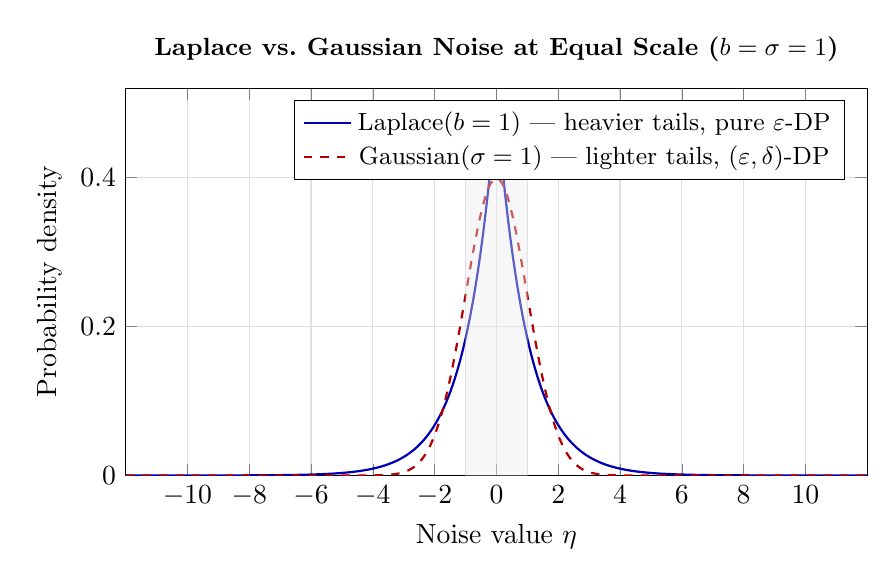
\begin{tikzpicture}
\begin{axis}[
  width=11cm, height=6.5cm,
  xlabel={Noise value $\eta$},
  ylabel={Probability density},
  xmin=-12, xmax=12,
  ymin=0,   ymax=0.52,
  xtick={-10,-8,-6,-4,-2,0,2,4,6,8,10},
  legend pos=north east,
  legend style={font=\small},
  grid=major, grid style={gray!25},
  title={Laplace vs.\ Gaussian Noise at Equal Scale ($b = \sigma = 1$)},
  title style={font=\small\bfseries}
]
% Laplace(0,1): f(x) = 0.5 * exp(-|x|)
\addplot[blue!70!black, thick, domain=-12:12, samples=300]
  { 0.5 * exp(-abs(x)) };
\addlegendentry{Laplace($b=1$) — heavier tails, pure $\varepsilon$-DP}

% Gaussian(0,1): f(x) = 1/sqrt(2pi) * exp(-x^2/2)
\addplot[red!70!black, thick, dashed, domain=-12:12, samples=300]
  { 1/sqrt(2*pi) * exp(-x^2/2) };
\addlegendentry{Gaussian($\sigma=1$) — lighter tails, $(\varepsilon,\delta)$-DP}

% Mark sensitivity region
\addplot[gray!60, fill=gray!15, opacity=0.4]
  coordinates {(-1,0)(-1,0.5)(1,0.5)(1,0)} -- cycle;
\node[font=\scriptsize, gray!70!black] at (axis cs:0,0.45)
  {$\Delta f = 1$};
\end{axis}
\end{tikzpicture}
\caption{Laplace vs.\ Gaussian noise distributions at unit scale. The Laplace mechanism has heavier tails (higher probability of large noise) but achieves pure $\varepsilon$-DP. The Gaussian mechanism has lighter tails, achieving $(\varepsilon, \delta)$-DP, and is preferred for deep learning because it composes more efficiently under the Moments Accountant.}
\label{fig:ch5_noise_comparison}
\end{figure}

\section{Privacy in Deep Learning: DP-SGD}
\label{sec:dp_sgd}

Standard Stochastic Gradient Descent (SGD) is vulnerable; an individual record's gradient can be extracted from the model's weights \cite{zhu2019}. \textbf{DP-SGD} (Differentially Private SGD) fixes this through two critical modifications at every training step:

\begin{enumerate}
    \item \textbf{Per-Sample Gradient Clipping:} Each individual gradient $\mathbf{g}_i = \nabla_\theta \mathcal{L}(\theta, x_i)$ is clipped to a maximum $\ell_2$ norm $C$, bounding the sensitivity of the sum:
    \begin{equation}
      \bar{\mathbf{g}}_i = \mathbf{g}_i \cdot \min\!\left(1,\; \frac{C}{\|\mathbf{g}_i\|_2}\right)
      \label{eq:dp_clipping}
    \end{equation}
    \item \textbf{Gaussian Noise Addition:} The batch sum of clipped gradients is noised before the optimizer step:
    \begin{equation}
      \tilde{\mathbf{g}} = \frac{1}{|B|}\left(\sum_{i \in B} \bar{\mathbf{g}}_i\right) + \mathcal{N}\!\left(\mathbf{0},\; \sigma^2 C^2 \mathbf{I}\right)
      \label{eq:dp_noise}
    \end{equation}
    where $\sigma$ is the \textbf{noise multiplier} — the key hyperparameter governing the privacy-utility trade-off.
\end{enumerate}

\subsection{The DP-SGD Algorithm}
\label{subsec:dpsgd_algorithm}

\begin{figure}[ht]
\centering
\begin{tikzpicture}[
  node distance=0.9cm and 2.2cm,
  font=\small,
  box/.style={draw, rounded corners=4pt, inner sep=8pt, text centered,
              minimum width=5.5cm, minimum height=1.0cm},
  privbox/.style={box, fill=blue!8, draw=blue!60!black},
  sgdbox/.style={box,  fill=gray!8,  draw=gray!60},
  noisebox/.style={box, fill=red!8,  draw=red!60!black},
  arrow/.style={->, >=Stealth, thick, gray!70}
]

\node (sample) [sgdbox,align=left]
    {\textbf{1. Sample mini-batch} $B \subset D$\\
     Poisson sampling rate $q = |B|/N$};

\node (clip) [privbox, below=of sample,align=left]
    {\textbf{2. Per-sample gradient clip}\\
     $\bar{\mathbf{g}}_i \leftarrow \mathbf{g}_i \cdot \min(1, C/\|\mathbf{g}_i\|_2)$\\
     \textit{(bounds sensitivity to $C$)}};

\node (noise) [noisebox, below=of clip,align=left]
    {\textbf{3. Add Gaussian noise}\\
     $\tilde{\mathbf{g}} \leftarrow \frac{1}{|B|}\!\sum \bar{\mathbf{g}}_i + \mathcal{N}(0, \sigma^2 C^2 \mathbf{I})$\\
     \textit{(DP guarantee injected here)}};

\node (update) [sgdbox, below=of noise,align=left]
    {\textbf{4. Optimizer step}\\
     $\theta \leftarrow \theta - \eta\,\tilde{\mathbf{g}}$};

\node (account) [privbox, right=2.2cm of noise, text width=4.5cm, align=center]
    {\textbf{Privacy Accountant}\\[4pt]
     Tracks cumulative $\varepsilon$\\
     via Rényi DP / GDP\\[4pt]
     Stops training when\\
     $\varepsilon_{\mathrm{consumed}} \geq \varepsilon_{\mathrm{budget}}$};

\draw [arrow] (sample.south) -- (clip.north);
\draw [arrow] (clip.south)   -- (noise.north);
\draw [arrow] (noise.south)  -- (update.north);
\draw [arrow] (update.west)  -- ++(-1.2,0) |- (sample.west)
    node[left, pos=0.25, font=\scriptsize] {next step};
\draw [arrow, dashed, blue!60] (noise.east) -- (account.west)
    node[above, font=\scriptsize, midway] {$\varepsilon$ increment};

\end{tikzpicture}
\caption{The DP-SGD training loop. Steps 1 and 4 are standard SGD; Steps 2 and 3 inject the differential privacy guarantee. The Privacy Accountant runs alongside the loop, halting training when the cumulative privacy budget is exhausted.}
\label{fig:dpsgd_loop}
\end{figure}

\subsection{Worked Example: DP-SGD Hyperparameter Calibration}
\label{subsec:dpsgd_example}

\textbf{Setting:} Train a fraud classifier on $N = 100{,}000$ transactions, target $(\varepsilon = 2.0,\, \delta = 10^{-5})$-DP after $T = 5{,}000$ steps, batch size $|B| = 256$.

\textbf{Sampling rate:} $q = 256/100{,}000 = 0.00256$.

\textbf{Noise multiplier:} Using the RDP accountant (available in Opacus \cite{opacus}), the noise multiplier $\sigma$ that achieves the target budget is approximately $\sigma \approx 1.1$ — meaning noise with standard deviation $1.1 \times C$ is added per step.

\textbf{Clipping norm:} A practical heuristic is to set $C$ at the median per-sample gradient norm of an unprotected pilot run. For this dataset, $C = 1.0$.

\textbf{Utility impact:} With these settings, the fraud classifier loses approximately 1.2 percentage points of AUC compared to the unprotected baseline — a commercially acceptable cost for a legally compliant system under GDPR Article 25 and Vietnam Decree 13.

\subsection{DP-SGD Implementation with Opacus}
\label{subsec:dpsgd_code}

\begin{lstlisting}[language=Python, style=pythonstyle,
  caption={DP-SGD training loop using Meta's Opacus library. The \texttt{make\_private()} call wraps the optimizer and model to enforce per-sample clipping and Gaussian noise injection automatically. The \texttt{get\_epsilon()} method queries the RDP accountant for the current cumulative privacy cost.},
  label={lst:dpsgd_opacus}]
import torch
from torch.utils.data import DataLoader
from opacus import PrivacyEngine
from opacus.validators import ModuleValidator

# --- 1. Model and data ------------------------------------------
model    = FraudClassifier()
model    = ModuleValidator.fix(model)  # replace incompatible layers
optimizer = torch.optim.Adam(model.parameters(), lr=1e-3)
train_loader = DataLoader(train_dataset, batch_size=256, shuffle=True)

# --- 2. Attach PrivacyEngine ------------------------------------
privacy_engine = PrivacyEngine()
model, optimizer, train_loader = privacy_engine.make_private_with_epsilon(
    module       = model,
    optimizer    = optimizer,
    data_loader  = train_loader,
    epochs       = 20,
    target_epsilon = 2.0,   # privacy budget
    target_delta   = 1e-5,
    max_grad_norm  = 1.0,   # clipping norm C
)
print(f"Noise multiplier sigma = {optimizer.noise_multiplier:.3f}")

# --- 3. Training loop -------------------------------------------
for epoch in range(20):
    for X_batch, y_batch in train_loader:
        optimizer.zero_grad()
        loss = criterion(model(X_batch), y_batch)
        loss.backward()
        optimizer.step()   # clipping + noise applied automatically

    eps = privacy_engine.get_epsilon(delta=1e-5)
    print(f"Epoch {epoch+1:02d} | loss={loss.item():.4f} | "
          f"eps consumed = {eps:.3f}")
    if eps >= 2.0:
        print("Privacy budget exhausted -- stopping training.")
        break
\end{lstlisting}

\section{Privacy Accounting and Composition}
\label{sec:dp_composition}

In deep learning, we query the data every single step. Privacy loss \textit{accumulates}. \textbf{Composition} is the study of how these small "leaks" add up over time. Modern architects use \textbf{Rényi Differential Privacy (RDP)} or \textbf{Gaussian DP (GDP)} to track this budget much more accurately than simple addition, enabling thousands of training steps while keeping $\epsilon$ under control.

\subsection{Why Naïve Composition Fails}
\label{subsec:naive_composition}

\textbf{Basic composition theorem:} If mechanism $M_1$ is $\varepsilon_1$-DP and $M_2$ is $\varepsilon_2$-DP, their sequential composition is $(\varepsilon_1 + \varepsilon_2)$-DP.

\textbf{The problem:} Applying this naïvely to DP-SGD with $T = 5{,}000$ steps and per-step $\varepsilon_{\text{step}} = 0.001$ gives $\varepsilon_{\text{total}} = 5.0$ — a very weak guarantee. RDP accountant tracks the \emph{actual} privacy loss under Poisson subsampling amplification, producing $\varepsilon_{\text{total}} \approx 2.0$ for the same run — a 2.5$\times$ improvement.

\subsection{Worked Example: Privacy Budget Ledger}
\label{subsec:budget_ledger}

Table~\ref{tab:budget_ledger} shows how a Privacy Budget Ledger tracks $\varepsilon$ consumption across the lifecycle of a medical AI system. Each operation consumes a portion of the total budget; the sum must remain below the approved ceiling.

\begin{table}[ht]
\centering
\caption{Privacy Budget Ledger: tracking $\varepsilon$ consumption across all operations on a medical dataset ($\varepsilon_{\mathrm{total}} = 4.0$, $\delta = 10^{-5}$). The ledger is an immutable audit record required by the Verifiability Pillar.}
\label{tab:budget_ledger}
\renewcommand{\arraystretch}{1.3}
\begin{tabular}{p{4.0cm} p{2.8cm} p{1.8cm} p{2.0cm}}
\hline\noalign{\smallskip}
\textbf{Operation} & \textbf{Mechanism} & \textbf{$\varepsilon$ cost} & \textbf{Running total} \\
\noalign{\smallskip}\svhline\noalign{\smallskip}
Prevalence query (diabetes count) & Laplace($b=1$) & 1.00 & 1.00 \\
Mean age of cohort & Laplace($b=2$) & 0.50 & 1.50 \\
Model training (DP-SGD, $T=3{,}000$, $\sigma=1.1$) & RDP accountant & 1.80 & 3.30 \\
Histogram release (comorbidities) & Laplace($b=5$) & 0.20 & 3.50 \\
\rowcolor{costmed}
Synthetic data validation (MIA audit) & Gaussian($\sigma=3$) & 0.30 & 3.80 \\
\rowcolor{costhigh}
\textbf{Remaining budget} & --- & \textbf{0.20} & \textbf{3.80 / 4.00} \\
\noalign{\smallskip}\hline\noalign{\smallskip}
\end{tabular}
\end{table}

\begin{svgraybox}
\textbf{Architect's Rule:} Reserve at least 10\% of the total $\varepsilon$ budget as an \textbf{emergency reserve} for unplanned queries (regulatory audits, incident investigations). In the example above, $\varepsilon_{\mathrm{reserve}} = 0.40$ should be held back, meaning operations should halt at $\varepsilon_{\mathrm{consumed}} = 3.60$, not $4.00$. The Privacy Budget Ledger enforces this automatically via a pre-commit threshold check before each query is executed.
\end{svgraybox}

% ------------------------------------------------------------------
\section{Private Aggregation of Teacher Ensembles (PATE)}
\label{sec:pate}
% ------------------------------------------------------------------

DP-SGD protects privacy by noising the \emph{gradients} during training. \textbf{PATE} \cite{papernot2017} takes a fundamentally different approach: it protects privacy by noising the \emph{labels} used to train a student model, keeping the sensitive training data completely out of the student's training loop. This makes PATE particularly powerful for scenarios where the sensitive data cannot be used directly for model training (e.g., patient records protected under HIPAA/Decree~13), but a surrogate \emph{public} dataset of unlabeled inputs is available.

\subsection{Architecture: Teachers, Noisy Voting, and the Student}
\label{subsec:pate_architecture}

\begin{figure}[ht]
\centering
\begin{tikzpicture}[
  node distance=1.0cm and 1.6cm,
  font=\small,
  teacher/.style={draw, rounded corners=3pt, fill=red!8, draw=red!60!black,
                  inner sep=7pt, text centered, minimum width=3.2cm,
                  minimum height=0.9cm},
  vote/.style={draw, rounded corners=3pt, fill=orange!10, draw=orange!70!black,
               inner sep=8pt, align=center, minimum width=5.5cm,
               minimum height=1.0cm},
  student/.style={draw, rounded corners=3pt, fill=blue!8, draw=blue!60!black,
                  inner sep=8pt, align=center, minimum width=5.5cm,
                  minimum height=1.0cm},
  data/.style={draw, rounded corners=3pt, fill=gray!10, draw=gray!60,
               inner sep=6pt, align=center, minimum width=3.2cm,
               minimum height=0.8cm},
  arrow/.style={->, >=Stealth, thick, gray!70},
  darrow/.style={arrow, dashed, blue!50}
]

%% Private data partitions
\node (d1) [data] {Partition $D_1$\\(sensitive)};
\node (d2) [data, right=0.4cm of d1] {Partition $D_2$\\(sensitive)};
\node (d3) [data, right=0.4cm of d2] {Partition $D_3$\\(sensitive)};
\node (ddots)[font=\small, right=0.3cm of d3] {$\cdots$};
\node (dn) [data, right=0.3cm of ddots] {Partition $D_n$\\(sensitive)};

%% Teacher models (trained on disjoint partitions)
\node (t1) [teacher, below=0.8cm of d1] {Teacher $M_1$};
\node (t2) [teacher, below=0.8cm of d2] {Teacher $M_2$};
\node (t3) [teacher, below=0.8cm of d3] {Teacher $M_3$};
\node (tn) [teacher, below=0.8cm of dn] {Teacher $M_n$};

%% Noisy voting aggregator
\node (vote_node) [vote, below=1.1cm of t2, xshift=1.5cm]
    {\textbf{Noisy Argmax (Laplace)} \\
     $\hat{y} = \arg\max_c \bigl[ n_c(\mathbf{x}) + \text{Lap}(1/\gamma) \bigr]$\\
     {\scriptsize $n_c$ = votes for class $c$}};

%% Public unlabeled data
\node (pub) [data, right=2.0cm of vote_node, yshift=0.2cm]
    {Public unlabeled\\dataset $D_{\mathrm{pub}}$};

%% Student model
\node (student_node) [student, below=1.1cm of vote_node]
    {\textbf{Student Model}\\
     Trained on $(D_{\mathrm{pub}},\, \hat{y})$ only\\
     \emph{Never sees sensitive data}};

%% Arrows: data → teachers
\draw [arrow] (d1.south) -- (t1.north);
\draw [arrow] (d2.south) -- (t2.north);
\draw [arrow] (d3.south) -- (t3.north);
\draw [arrow] (dn.south) -- (tn.north);

%% Arrows: teachers → noisy vote
\draw [arrow] (t1.south) -- ++(0,-0.3) -| (vote_node.north);
\draw [arrow] (t2.south) -- (vote_node.north);
\draw [arrow] (t3.south) -- ++(0,-0.3) -| (vote_node.north);
\draw [arrow] (tn.south) -- ++(0,-0.3) -| (vote_node.north);

%% Public data → voting aggregator
\draw [arrow] (pub.west)  -- (vote_node.east)
    node[above, font=\scriptsize, midway] {query $\mathbf{x}$};

%% Noisy vote → student
\draw [arrow] (vote_node.south) -- (student_node.north)
    node[right, font=\scriptsize, midway] {noisy label $\hat{y}$};

%% Privacy boundary annotation
\draw [statered, dashed, line width=1.2pt]
    (-0.2, -1.5) rectangle (10.8, 0.7);
\node [font=\scriptsize\bfseries, statered] at (5.3, 0.5)
    {Privacy boundary: sensitive data never crosses below this line};

\end{tikzpicture}
\caption{PATE architecture. $n$ teacher models are trained on disjoint partitions of the sensitive dataset. For each unlabeled public query $\mathbf{x}$, teachers vote and the noisy argmax (Laplace noise) produces a private label $\hat{y}$. The student trains only on $(D_{\mathrm{pub}}, \hat{y})$ — the sensitive data never participates in student training.}
\label{fig:pate_architecture}
\end{figure}

\subsection{The Noisy Argmax Mechanism}
\label{subsec:pate_mechanism}

For a public query $\mathbf{x}$, each teacher $M_k$ votes for a class $c$. Let $n_c(\mathbf{x})$ be the vote count for class $c$. The \textbf{PATE noisy argmax} adds Laplace noise to each vote count before selecting the winner:
\begin{equation}
  \hat{y} = \arg\max_{c \in \mathcal{Y}} \bigl[ n_c(\mathbf{x}) + \eta_c \bigr], \quad
  \eta_c \sim \text{Lap}\!\left(\tfrac{1}{\gamma}\right)
  \label{eq:pate_noisy_argmax}
\end{equation}
where $\gamma > 0$ is the \textbf{voting privacy parameter}. The key insight is that the privacy cost is paid \emph{once per query to the teacher ensemble}, not once per training step — making PATE highly efficient when $|D_{\mathrm{pub}}|$ is small.

\textbf{Worked example.}
Three teachers vote on a public medical image (\textit{is this a malignant nodule?}). True vote counts: $n_{\mathrm{yes}} = 8$, $n_{\mathrm{no}} = 2$.  With $\gamma = 0.5$ (noise scale $= 1/\gamma = 2$), noise samples: $\eta_{\mathrm{yes}} = +1.3$, $\eta_{\mathrm{no}} = -0.7$.  Noisy counts: $9.3$ vs. $1.3$. The majority opinion survives the noise, as expected when consensus is strong. When the true vote is close (e.g., $6$ vs. $4$), the noise occasionally flips the label — this is the deliberate privacy cost.

\subsection{Privacy Guarantee and Comparison with DP-SGD}
\label{subsec:pate_privacy}

PATE's privacy guarantee is derived from the \emph{data-dependent privacy analysis}: if a large fraction of teachers agree on the correct label (high consensus), the noise is unlikely to flip the outcome, and the privacy cost per query is low. Semi-supervised PATE achieves $(0.59, 10^{-5})$-DP on MNIST with 98.5\% accuracy \cite{papernot2017} — state-of-the-art at that privacy level.

\begin{table}[ht]
\centering
\caption{DP-SGD vs.\ PATE: when to use each framework.}
\label{tab:dpsgd_vs_pate}
\begin{tabular}{p{4.0cm} p{4.5cm} p{4.5cm}}
\hline\noalign{\smallskip}
\textbf{Criterion} & \textbf{DP-SGD} & \textbf{PATE} \\
\noalign{\smallskip}\svhline\noalign{\smallskip}
Privacy mechanism & Gradient clipping + Gaussian noise per step & Noisy voting on teacher ensemble per query \\[3pt]
Sensitive data access & Model trains directly on sensitive data & Student \emph{never} touches sensitive data \\[3pt]
Public data required & No & Yes ($D_{\mathrm{pub}}$ of unlabeled inputs) \\[3pt]
Privacy accounting & Moments Accountant / RDP (complex) & Data-dependent analysis (intuitive) \\[3pt]
Best for & Large sensitive datasets; end-to-end training & Sensitive data scarce; public proxy data available; regulatory separation required \\[3pt]
Interpretability & Low (noise inside training) & High (explainable teacher vote counts) \\
\noalign{\smallskip}\hline\noalign{\smallskip}
\end{tabular}
\end{table}

\subsection{PATE Implementation}
\label{subsec:pate_code}

\begin{lstlisting}[language=Python, style=pythonstyle,
  caption={PATE framework: teacher ensemble training on disjoint data partitions, noisy argmax aggregation, and student training on public data with private labels. The \texttt{privacy\_cost()} function implements the basic data-independent RDP bound; production deployments should use the tight data-dependent bound from the \texttt{autodp} library.},
  label={lst:pate_implementation}]
import numpy as np
from sklearn.base import clone

# --- 1. Train n teachers on disjoint partitions -----------------
def train_teachers(base_model, X_priv, y_priv, n_teachers):
    """Split sensitive data into n disjoint partitions; train one teacher each."""
    teachers = []
    partitions = np.array_split(np.arange(len(X_priv)), n_teachers)
    for idx in partitions:
        m = clone(base_model).fit(X_priv[idx], y_priv[idx])
        teachers.append(m)
    return teachers

# --- 2. Noisy argmax on public queries --------------------------
def noisy_argmax(teachers, X_pub, n_classes, gamma=0.5):
    """
    For each public query: aggregate teacher votes, add Laplace noise,
    return private label.  gamma controls noise scale (higher = more private).
    Returns private labels and per-query max-vote fraction (for analysis).
    """
    private_labels = []
    consensus_scores = []
    for x in X_pub:
        votes = np.zeros(n_classes)
        for teacher in teachers:
            pred = teacher.predict([x])[0]
            votes[int(pred)] += 1
        noise  = np.random.laplace(0, 1.0 / gamma, size=n_classes)
        noisy  = votes + noise
        label  = int(np.argmax(noisy))
        private_labels.append(label)
        consensus_scores.append(votes.max() / len(teachers))
    return np.array(private_labels), np.array(consensus_scores)

# --- 3. Train student on public data + private labels -----------
def train_student(student_model, X_pub, private_labels):
    """Student only ever sees (public_input, noisy_label) pairs."""
    return clone(student_model).fit(X_pub, private_labels)

# --- 4. Privacy cost estimate (data-independent RDP bound) ------
def privacy_cost(n_queries, gamma, delta=1e-5):
    """
    Approximate epsilon using the moments accountant bound.
    For tight bounds, use the autodp library with data-dependent analysis.
    """
    # RDP order alpha=2 bound for Laplace noise with parameter 1/gamma
    rdp_per_query = gamma**2 / 2.0
    rdp_total     = rdp_per_query * n_queries
    # Convert RDP to (epsilon, delta)-DP
    epsilon = rdp_total + np.sqrt(2 * rdp_total * np.log(1 / delta))
    return epsilon

# --- Example usage ----------------------------------------------
if __name__ == "__main__":
    from sklearn.ensemble import RandomForestClassifier

    base    = RandomForestClassifier(n_estimators=50, random_state=0)
    N_TEACH = 50;   N_CLASSES = 2;   GAMMA = 0.5

    teachers = train_teachers(base, X_sensitive, y_sensitive, N_TEACH)

    private_labels, consensus = noisy_argmax(
        teachers, X_public_unlabeled, N_CLASSES, gamma=GAMMA)

    # Only train student when consensus is high (reduces privacy cost)
    high_conf = consensus >= 0.7
    student = train_student(base, X_public_unlabeled[high_conf],
                            private_labels[high_conf])

    eps = privacy_cost(n_queries=high_conf.sum(), gamma=GAMMA)
    print(f"Labels used: {high_conf.sum()} | Estimated eps = {eps:.3f}")
    print(f"Student accuracy: {student.score(X_test, y_test):.3%}")
\end{lstlisting}

\begin{svgraybox}
\textbf{When to Choose PATE over DP-SGD:} If your regulatory context requires that the sensitive dataset \emph{never participates in model training} (a common interpretation of data minimization under GDPR Article 5 and Vietnam Decree 13 Article 6), PATE satisfies this requirement by design. DP-SGD does not: the sensitive data is directly consumed in the gradient computation. For healthcare and biometric applications subject to the strictest data handling requirements, PATE's architectural separation is often the legally superior choice even when its statistical efficiency is lower.
\end{svgraybox}

% ------------------------------------------------------------------
\subsection{DP-SGD Hyperparameter Selection Guide}
\label{subsec:dpsgd_hyperparams}
% ------------------------------------------------------------------

Knowing \emph{how} DP-SGD works is necessary; knowing \emph{which hyperparameters to choose} is the practitioner's first bottleneck. The three key parameters --- clipping norm $C$, noise multiplier $\sigma$, and batch size $B$ --- jointly determine both the privacy cost and the accuracy loss. Table~\ref{tab:dpsgd_hyperparams} provides empirically calibrated starting points for the four most common deployment scenarios.

\begin{table}[ht]
\centering
\caption{DP-SGD Hyperparameter Starting Points by deployment scenario. $\varepsilon$ values are estimated at $\delta = 10^{-5}$ using the RDP accountant (Opacus). All values assume 20 training epochs; halving epochs approximately halves $\varepsilon$ at constant $\sigma$.}
\label{tab:dpsgd_hyperparams}
\renewcommand{\arraystretch}{1.3}
\begin{tabular}{p{2.8cm} p{1.5cm} p{1.5cm} p{1.2cm} p{1.8cm} p{3.5cm}}
\hline\noalign{\smallskip}
\textbf{Scenario} & \textbf{$C$ (clip)} & \textbf{$\sigma$} & \textbf{$B$} & \textbf{Est.\ $\varepsilon$ (20 ep.)} & \textbf{Expected Accuracy Drop} \\
\noalign{\smallskip}\svhline\noalign{\smallskip}
Small sensitive dataset ($N\!\leq\!5{,}000$), Class A & \cellcolor{costhigh}1.0 & \cellcolor{costhigh}2.0 & 64 & \cellcolor{costhigh}$\approx 1.0$ & \cellcolor{costhigh}$-8$\% to $-15$\% \\[3pt]
Medium dataset ($N\!\approx\!50{,}000$), Class B & 1.0 & 1.5 & 256 & \cellcolor{costmed}$\approx 2.0$ & $-3$\% to $-8$\% \\[3pt]
Large dataset ($N\!\geq\!500{,}000$), Class C & 1.0 & 1.1 & 512 & \cellcolor{costlow}$\approx 4.0$ & $-1$\% to $-3$\% \\[3pt]
Fine-tuning only (LoRA, rank 16), any $N$ & 0.5 & 1.5 & 256 & \cellcolor{costmed}$\approx 2.0$ & $-1$\% to $-4$\% (LoRA adapters only) \\
\noalign{\smallskip}\hline\noalign{\smallskip}
\end{tabular}
\end{table}

\begin{svgraybox}
\textbf{Tuning Priority Order:} (1)~Set $\sigma$ first --- it is the primary lever for $\varepsilon$. (2)~Increase $B$ (larger batch = fewer steps = less accumulated noise at same $\varepsilon$). (3)~Lower $C$ only if gradient norms are already near 1.0 (check with a non-private trial run). Never lower $C$ below 0.5 without measuring the resulting accuracy drop on a validation set. Reserve the 10\% budget margin (Section~\ref{subsec:budget_ledger}) before finalizing parameters.
\end{svgraybox}

% ------------------------------------------------------------------
\section{Local Differential Privacy: When the Server Cannot Be Trusted}
\label{sec:ldp}
% ------------------------------------------------------------------

The DP-SGD framework of Section~\ref{sec:dp_sgd} operates under a \textbf{central trust model}: the aggregation server is assumed honest. In \textbf{Southeast Asian mobile-first economies}, many deployments involve consumer-device data collection through third-party analytics servers that may be untrustworthy, foreign-operated, or subject to a different jurisdiction's lawful-access regime.

\textbf{Local Differential Privacy (LDP)} shifts noise injection from the server to the \textbf{device itself}. A user's data is perturbed \emph{before} it leaves their device. The server receives only the noisy response and can never reconstruct the original input---even with unlimited computational resources.

\subsection{The Randomized Response Mechanism}
\label{subsec:randomized_response}

The canonical LDP primitive is \textbf{Randomized Response} \cite{warner1965}. For a binary attribute $b \in \{0, 1\}$, the $\varepsilon$-LDP mechanism outputs:

\begin{equation}
\mathcal{M}_\varepsilon(b) =
\begin{cases}
b       & \text{with probability } p = \dfrac{e^\varepsilon}{1 + e^\varepsilon} \\[6pt]
1 - b   & \text{with probability } 1 - p = \dfrac{1}{1 + e^\varepsilon}
\end{cases}
\label{eq:randomized_response}
\end{equation}

The server aggregates $n$ noisy reports and de-biases to estimate the true proportion. For high-cardinality categorical features, \textbf{OLH (Optimized Local Hashing)} and Google's \textbf{RAPPOR} protocol extend Randomized Response to practical feature spaces.

\subsection{The Utility Cost and the Trust Trade-off}
\label{subsec:ldp_utility}

The fundamental trade-off between LDP and central DP is a statistical efficiency gap of $O(\sqrt{n})$: achieving the same estimation accuracy under LDP requires approximately $n$ times more data than under central DP for the same $\varepsilon$.

\begin{description}
  \item[Central DP (server trusted):] Noise $\propto 1/n$; high utility at small $n$; server sees raw individual reports before noise.
  \item[LDP (server untrusted):] Noise $\propto 1/\sqrt{n}$; requires large $n$ (millions of users) for high utility; server only ever sees noisy reports.
\end{description}

\begin{svgraybox}
\textbf{Mobile Deployment Pattern (Vietnam, 2026):} For a consumer app collecting location-sensitive behavioral telemetry, the recommended architecture is \textbf{Double-DP}: (1) apply $\varepsilon_\mathrm{local} = 1.0$ LDP on-device using OLH before any network transmission; (2) apply an additional $\varepsilon_\mathrm{central} = 0.5$ DP-SGD layer at model training. This satisfies Decree 356's on-device privacy requirement while maintaining acceptable model utility at the scale of Vietnam's 70M+ mobile user base.
\end{svgraybox}

\section{Conclusion}
\label{sec:conclusion_dp}

Differential Privacy is the only framework that provides a provable guarantee against future attackers with arbitrary background knowledge. This chapter established the full DP toolkit available to the Trustworthy AI Architect:

\begin{description}
  \item[Laplace and Gaussian Mechanisms] for releasing statistical queries with calibrated noise, as shown in the worked examples of Sections~\ref{subsec:laplace_example} and~\ref{subsec:gaussian_example}.
  \item[DP-SGD] for training deep models directly on sensitive data, with per-sample gradient clipping, Gaussian noise injection, and RDP accounting tracked via the Opacus library.
  \item[Privacy Budget Ledger] for managing cumulative $\varepsilon$ consumption across the full AI lifecycle, with a 10\% emergency reserve.
  \item[PATE] for scenarios where regulatory or legal requirements demand that sensitive data \emph{never participate in model training} — the student model learns from noisy teacher votes on public data, achieving strong privacy guarantees with an interpretable, auditable architecture.
  \item[Local DP] for untrusted-server deployments where noise must be injected on-device before any network transmission.
\end{description}

A shield is only useful if we know what we are defending against. In the next chapter, we look at the specific attacks---from Membership Inference and Evasion to Data Poisoning and Model Extraction---that target the vulnerabilities DP is designed to close, and pair each attack with its architectural countermeasure.


